\documentclass[12pt]{article}%

\usepackage{amsmath,amssymb}
\usepackage{lmodern}
\usepackage{ifxetex,ifluatex}
\ifnum 0\ifxetex 1\fi\ifluatex 1\fi=0 % if pdftex
  \usepackage[T1]{fontenc}
  \usepackage[utf8]{inputenc}
  \usepackage{textcomp} % provide euro and other symbols
\else % if luatex or xetex
  \usepackage{unicode-math}
  \defaultfontfeatures{Scale=MatchLowercase}
  \defaultfontfeatures[\rmfamily]{Ligatures=TeX,Scale=1}
\fi
% Use upquote if available, for straight quotes in verbatim environments
\IfFileExists{upquote.sty}{\usepackage{upquote}}{}
\IfFileExists{microtype.sty}{% use microtype if available
  \usepackage[]{microtype}
  \UseMicrotypeSet[protrusion]{basicmath} % disable protrusion for tt fonts
}{}
\makeatletter
\@ifundefined{KOMAClassName}{% if non-KOMA class
  \IfFileExists{parskip.sty}{%
    \usepackage{parskip}
  }{% else
    \setlength{\parindent}{0pt}
    \setlength{\parskip}{6pt plus 2pt minus 1pt}}
}{% if KOMA class
  \KOMAoptions{parskip=half}}
\makeatother
\usepackage{xcolor}
\IfFileExists{xurl.sty}{\usepackage{xurl}}{} % add URL line breaks if available
\IfFileExists{bookmark.sty}{\usepackage{bookmark}}{\usepackage{hyperref}}
\hypersetup{
  pdftitle={Enrollment regression},
  pdfauthor={Ahmed},
  hidelinks,
  pdfcreator={LaTeX via pandoc}}
\urlstyle{same} % disable monospaced font for URLs
\usepackage[margin=1in]{geometry}
\usepackage{longtable,booktabs,array}
\usepackage{calc} % for calculating minipage widths
% Correct order of tables after \paragraph or \subparagraph
\usepackage{etoolbox}
\makeatletter
\patchcmd\longtable{\par}{\if@noskipsec\mbox{}\fi\par}{}{}
\makeatother
% Allow footnotes in longtable head/foot
\IfFileExists{footnotehyper.sty}{\usepackage{footnotehyper}}{\usepackage{footnote}}
\makesavenoteenv{longtable}
\usepackage{graphicx}
\makeatletter
\def\maxwidth{\ifdim\Gin@nat@width>\linewidth\linewidth\else\Gin@nat@width\fi}
\def\maxheight{\ifdim\Gin@nat@height>\textheight\textheight\else\Gin@nat@height\fi}
\makeatother
% Scale images if necessary, so that they will not overflow the page
% margins by default, and it is still possible to overwrite the defaults
% using explicit options in \includegraphics[width, height, ...]{}
\setkeys{Gin}{width=\maxwidth,height=\maxheight,keepaspectratio}
% Set default figure placement to htbp
\makeatletter
\def\fps@figure{htbp}
\makeatother
\setlength{\emergencystretch}{3em} % prevent overfull lines
\providecommand{\tightlist}{%
  \setlength{\itemsep}{0pt}\setlength{\parskip}{0pt}}
\setcounter{secnumdepth}{-\maxdimen} % remove section numbering
\usepackage{booktabs}
\usepackage{longtable}
\usepackage{array}
\usepackage{multirow}
\usepackage{wrapfig}
\usepackage{float}
\usepackage{colortbl}
\usepackage{pdflscape}
\usepackage{tabu}
\usepackage{threeparttable}
\usepackage{threeparttablex}
\usepackage[normalem]{ulem}
\usepackage{makecell}
\usepackage{xcolor}
\ifluatex
  \usepackage{selnolig}  % disable illegal ligatures
\fi
\usepackage{subcaption}
\begin{document}




%%%%%%%%%%%%%%%%%
% 2 side by side
%%%%%%%%%%%%%%%%%
\FloatBarrier
\begin{figure}
    \caption{Marijuana consumption indicator by legalization status}
     \label{fig:mari_consumpt}
                 \begin{subfigure}[H]{0.49\textwidth}
                     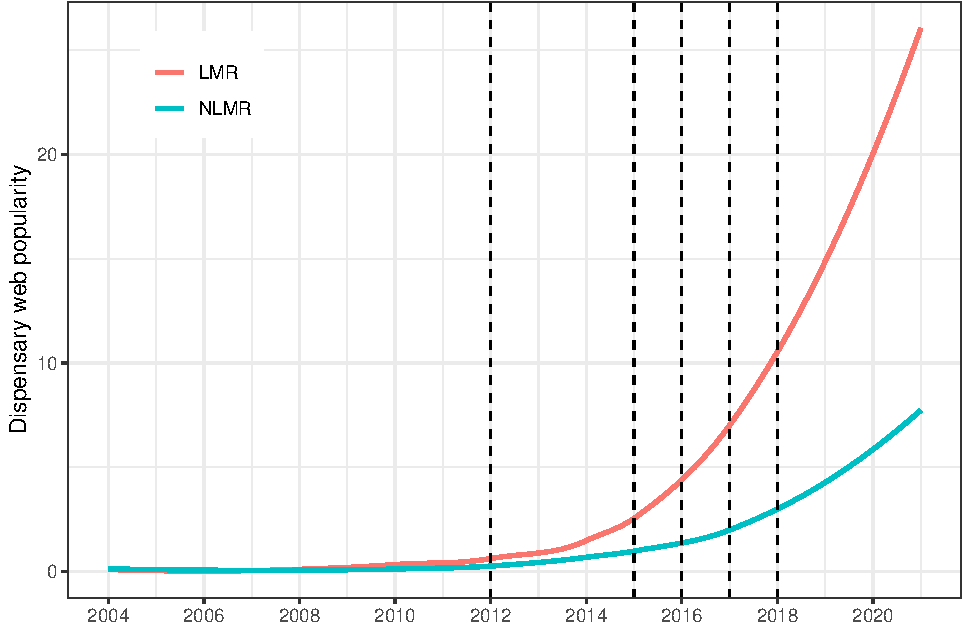
\includegraphics[width=\textwidth]{figures/disp_group.pdf}
                     \caption{}
                 \end{subfigure}
     \hfill
             \begin{subfigure}[H]{0.48\textwidth}
                 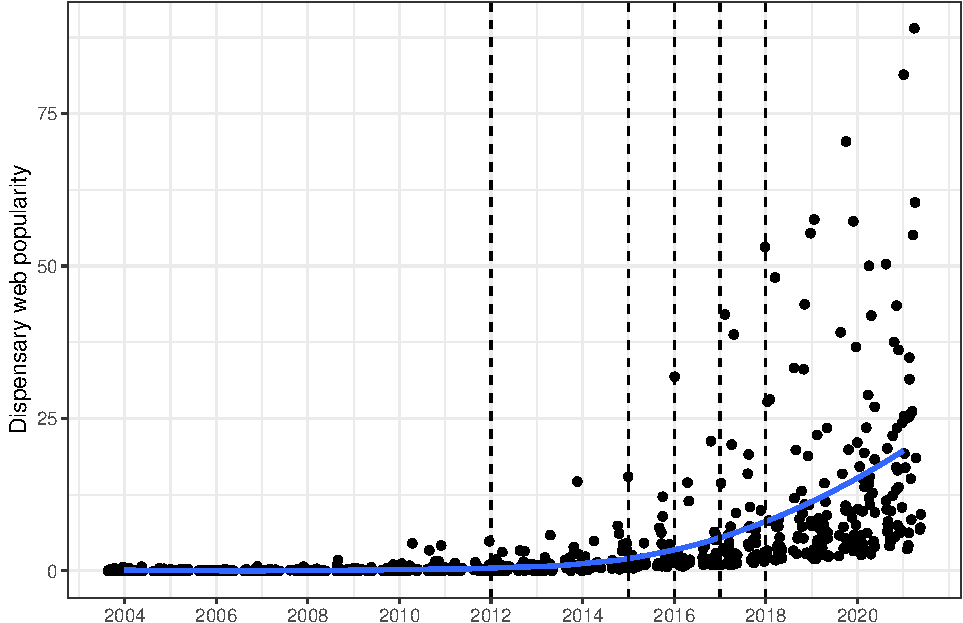
\includegraphics[width=\textwidth]{figures/disp.pdf}
                  \caption{}
             \end{subfigure}
\scriptsize 
\floatfoot{\textit{Note:}  The vertical lines refer to the time period in which a state legalized marijuana for recreational use (LMR) ; for instance, Washington and Colorado LMR in 2012. Google web popularity \footnotemark   (refer to as hits in google trend) is a number between 0 and 100 that measures the popularity of google search terms or words, showing how popular a word is among all other searches in particular region and time. In figure (a), we took the average of google web popularity for both states that LMR and those that didn't legalized marijuana for recreational use (NLMR). Also, note that NLMR include states that legalized marijuana for medical use which explains why NLMR have an increasing but smaller web popularity for dispensary compared to LMR states. } 

\end{figure}
\FloatBarrier
\footnotetext{We extracted  google trend data via 'gtrendsR', an R library. Data source: Google Trends (https://www.google.com/trends)} 
%%%%%%%%%%%%%%%%%%%%%%%%%%%%%%%

%%%%%%%%%%%%%%%%%
% 2 side by side
%%%%%%%%%%%%%%%%%
\FloatBarrier
\begin{figure}
    \caption{Common trend }
    \label{fig:trend}
                 \begin{subfigure}[H]{0.49\textwidth}
                     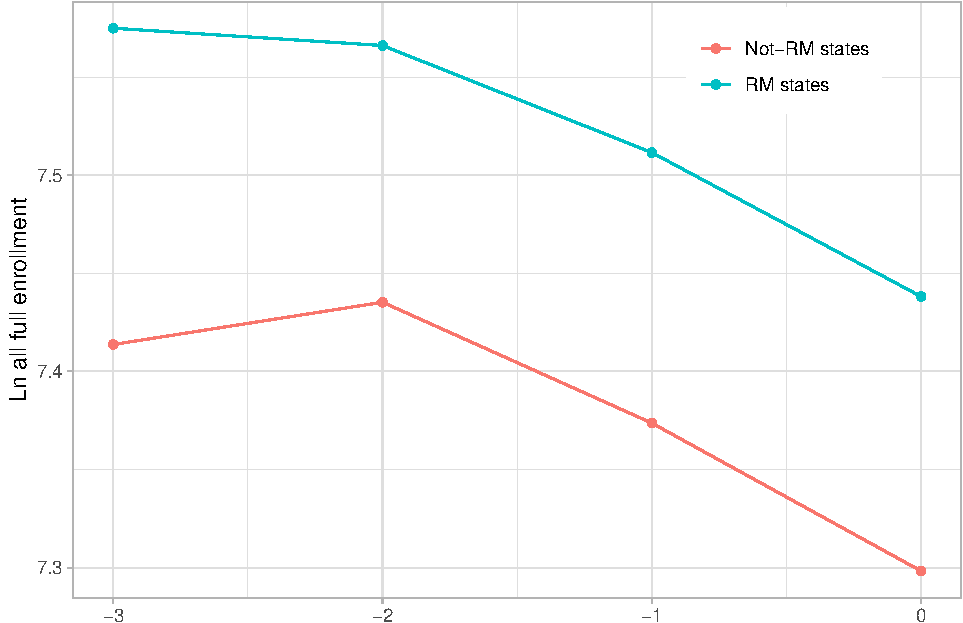
\includegraphics[width=\textwidth]{figures/ct1.pdf}
                     \caption{}
                 \end{subfigure}
     \hfill
             \begin{subfigure}[H]{0.48\textwidth}
                 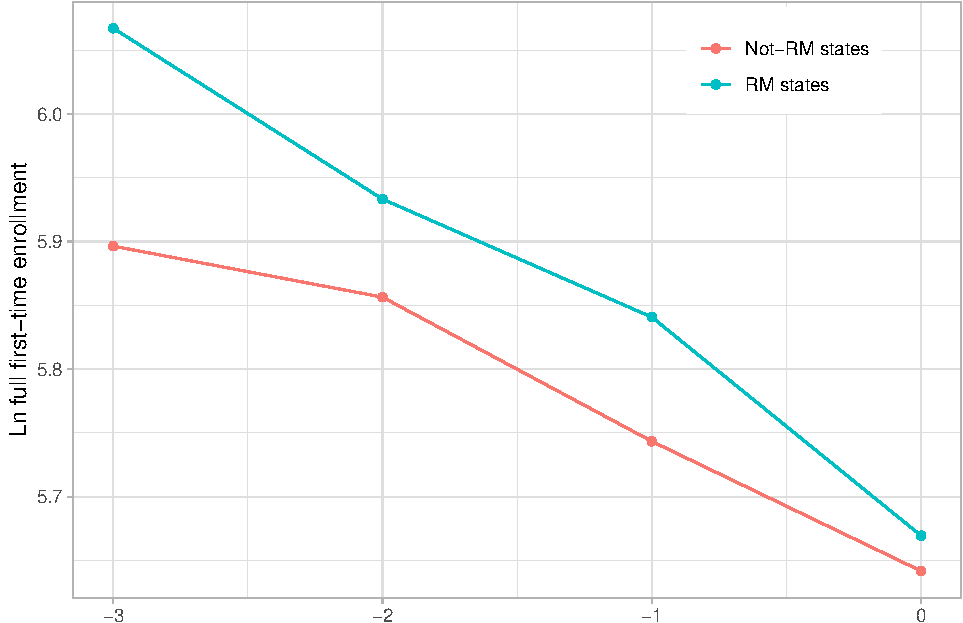
\includegraphics[width=\textwidth]{figures/ct2.pdf}
                  \caption{}
             \end{subfigure}
\scriptsize 
\floatfoot{\textit{Note:}  In the x-axis, zero refers to 2012, the first year in which RM is first legalized by Colorado and Washington states. The plots show that common trend  nearly holds before the policy shock for both first time and all undergraduate enrollments.   } 
 \label{fig:mari_consumpt}
\end{figure}


%%%%%%%%%%%%%%%%%%%%%%%%%%%%%%%
\newpage
\FloatBarrier
%::::::::::::::::::::::::
% motivation #1; only the aggregated mean
%::::::::::::::::::::::::::::::::::::::::

\FloatBarrier
\begin{figure}[htbp]

\caption{ }
\label{fig:drug}
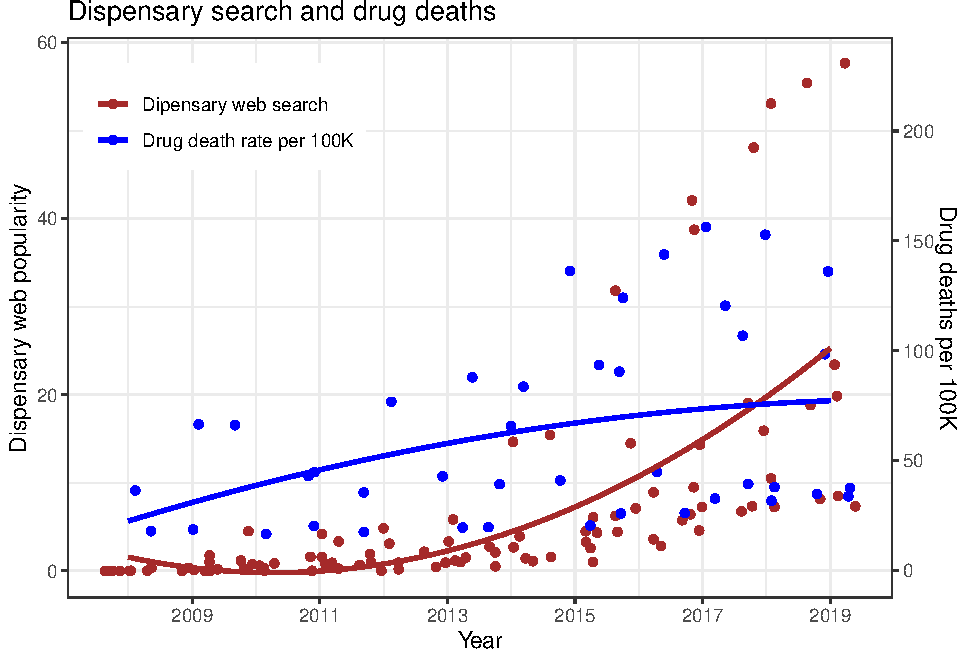
\includegraphics{figures/death_dispensary.pdf}
\floatfoot{\textit{Note:}   The figure illustrates an existing positive association between web search for \href{https://trends.google.com/trends/?geo=US}{dispensary}\footnotemark    (marijuana consumption proxy) and drug related deaths per 100K \footnotemark. Whereas the point show the actual measures, the lines represent the quadratic linear fit or trend.}
\end{figure}
\FloatBarrier


\footnotetext{We extracted  google trend data via 'gtrendsR', an R library. Data source: Google Trends (https://www.google.com/trends)} 

\footnote{ We extracted the drug mortality for age groups 15 to 34 from CDC \href{https://wonder.cdc.gov/ucd-icd10.html}{CDC WONDER database} \citep{cdcdata}}


%::::::::::::::::::::::::
% marijuana legalization
%::::::::::::::::::::::::::::::::::::::::

\FloatBarrier
\begin{figure}[htbp]

\caption{ Marijuana legalization timeline }
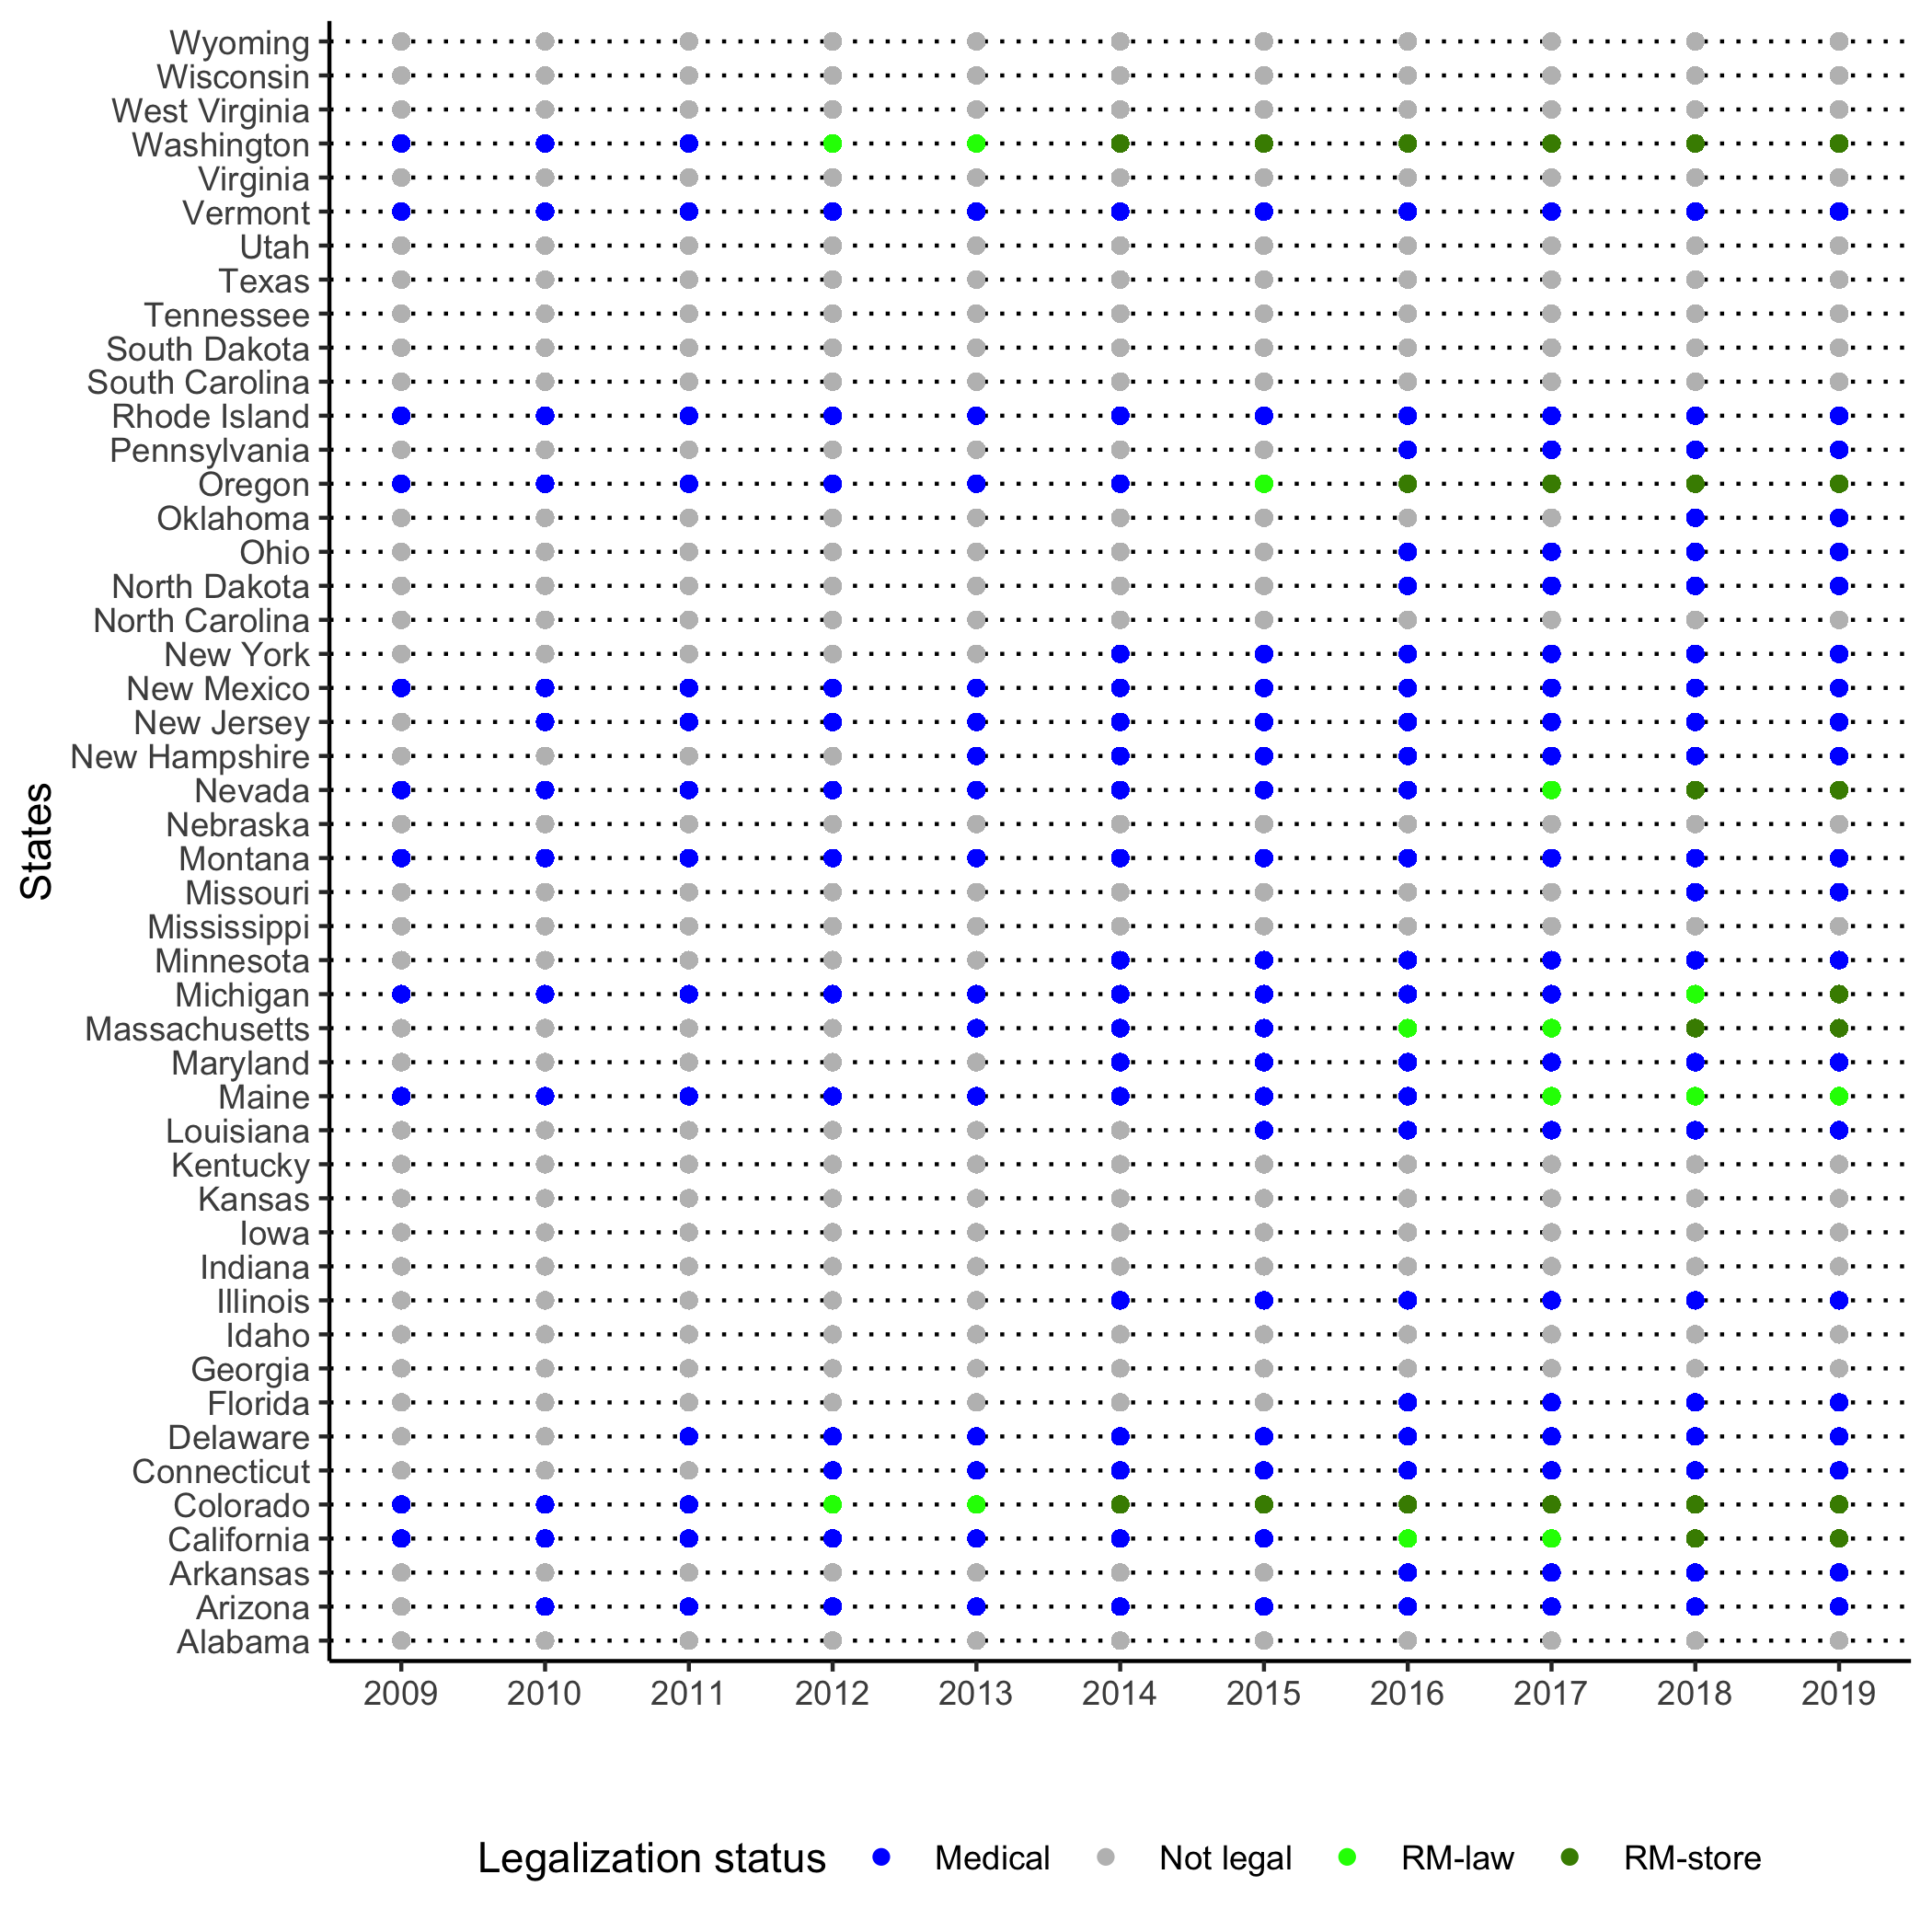
\includegraphics[width=\textwidth]{figures/mrl3.png}
\scriptsize 
\floatfoot{\textit{Note:}  The gaps depict transition from one status of legalization to another. DC, Arizona and all US territories are excluded due to either not sharing borders or unavailability of county and enrollment data.} 
 \label{fig:legal}
\end{figure}
\FloatBarrier

%::::::::::::::::::::::::::::::::::::::::



\end{document}